\documentclass[12pt]{article}

\usepackage{graphicx}

\title{CS 496 Lab 3: HTTP}
\author{Ian Kronquist}

\begin{document}
\maketitle

\begin{enumerate}
    \item The IP address of my browser client is 10.1.10.225. Its port number is 54072.
    \item The IP address of the server is 128.119.245.12. Its port number is 80.
    \item My client uses the ip, port pair of 10.1.10.225 and 54072.
    \item The sequence number of the TCP SYN segment is 0. The SYN flag is set to identify it as a SYN packet.
\begin{figure}[!ht]
    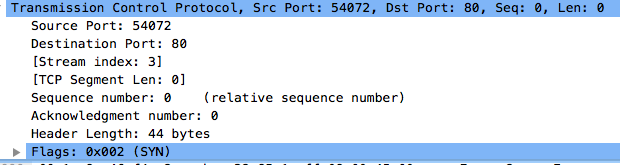
\includegraphics[scale=0.5]{./synpacket.png}
    \caption{SYN Packet}
\end{figure}


    \item The sequence number of the SYNACK segment is 1. The acknowledgement value is 1. The acknowledgement value was determined by adding 1 to then SYN segment sequence number. The flags for this segment are set to 0x12, identifying it as a SYNACK segment.
    \item The sequence number of the packet with the POST command is also 1.
    \item Table of information about the first 6 segments, including ACKs. Time is measured since the capture began. ACKs cannot have ACK received times, round trip times, or EstimatedRTT.



        $\texttt{EstimatedRTT} = (1 - \alpha ) \times \texttt{EstimatedRTT} + \alpha \times \texttt{SampleRTT}$, where $\alpha = 0.125$.


        \begin{table}[h]
            \centering
            \begin{tabular}{ p{1cm} | p{1.5cm} | p{1.5cm} | p{2.5cm} | p{2.5cm} | p{1.5cm}}
            Packet & Sequence Number & Sent Time & ACK Received time & Actual Round Trip Time & EstimatedRTT \\
            \hline
            1      & 1               & 2.391542    & 2.407970        & 0.016428               & 0.016428 \\
            2      & 1449            & 2.391543    & 2.407970        & 0.016430               & 0.016428 \\
            3      & 2897            & 2.391544    & 2.407973        & 0.016476               & 0.016434 \\
                4      & 1               & 2.407970    & N/A (ACK)       & N/A (ACK)                 & N/A (ACK) \\
                5      & 1               & 2.407973    & N/A (ACK)       & N/A (ACK)                 & N/A (ACK) \\
                6      & 1               & 2.408020    & N/A (ACK)       & N/A (ACK)                 & N/A (ACK) \\
        \end{tabular}
    \end{table}
    \item The lengths of the first 6 TCP segments are 1448, 1448, 1448, 0, 0, 0. Note that this does not include the TCP segment headers.
    \item The maximum segment size is 1460. This caused the sender to send smaller segments. I believe that the sender did throttle its output to prevent the receiver from dropping packets.
    \item No, there were no retransmitted packets. I checked by looking at the sequence numbers of the client's packets, ordered by time. Since there were no duplicates, and their sequence numbers only increased, there were no resubmitted packets. I also used the \texttt{tcp.analysis.retransmission} filter and it showed no retransmitted packets.
    \item In my capture, packet number 71 (ACK number 5793) acknowledges both packets 64 (Sequence number 4345) and 65 (Sequence number 5793). In most of the packets in my capture, ACKs only acknowledge individual segments.
    \item Throughput is measured in bytes over time. The connection started at time 2.373419 and ended at 2.513759, lasting a total of 0.14035 seconds. I could try to look at the total size of the file, add the total size of the headers, and count retransmissions, but Wireshark offers a very handy tool to do this for me. The average throughput but the end of the connection is just about $10^7$ bytes per second.
\begin{figure}[!ht]
    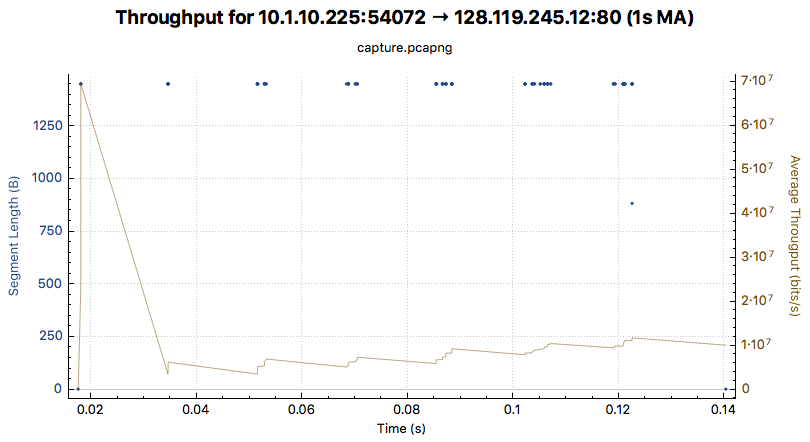
\includegraphics[scale=0.5]{./throughput.png}
    \caption{Throughput graph}
\end{figure}


    \item The TCP connection starts in slow start mode and continues to probe the network to try to find the congestion window by doubling the congestion window very ACK until congestion is encountered. This happens for the first 11 packets, or around 0.07816 seconds. It then switches to congestion avoidance mode until around packet 30 at 0.5767 seconds at which point it holds nearly the current transmission rate for the rest of the connection.
    \item For my connection it is not as clear cut. I believe it stayed in slow start mode for around the first 146 packets or around $2.462-2.373=0.0890$ seconds. It then enters congestion avoidance mode until around packet 185 at 0.108 seconds. However, the connection was closed around 0.01 seconds later, so it's hard to tell if it did leave congestion avoidance mode and enter a stable state.
\begin{figure}[!ht]
    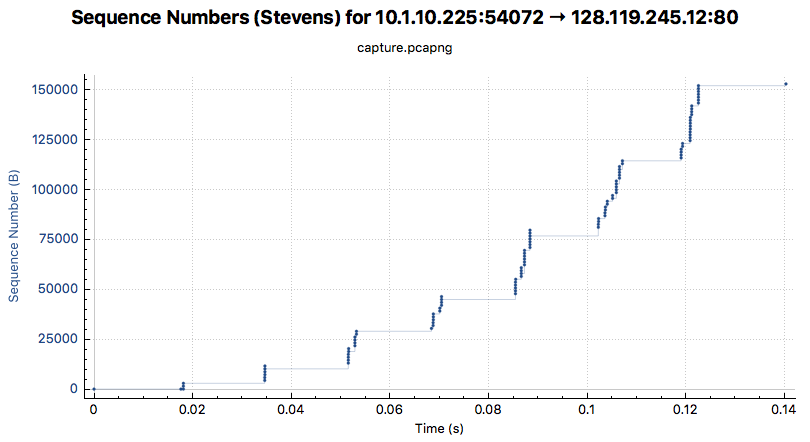
\includegraphics[scale=0.5]{./stevens.png}
    \caption{Stevens graph}
\end{figure}


\end{enumerate}

\end{document}
